\section{Training \& Inference Infrastructure}

\subsection{Pretraining}

We adopt Megatron-LM~\citep{megatron-lm} as the pretraining backend to enable efficient training of a 100B-parameter model with long sequences, leveraging data parallelism (DP), pipeline parallelism (PP), tensor parallelism (TP), context parallelism (CP), and expert parallelism (EP), as Figure \ref{fig:megatron_parallelism} shows. To ensure consistency of masked tokens, we generate masked tokens on a single model-parallel (MP, that is, TP and PP) rank and then broadcast to all other ranks within the MP ranks.

\begin{wrapfigure}{r}{0.5\textwidth}
    \centering
    \vspace{-1pt}  %
    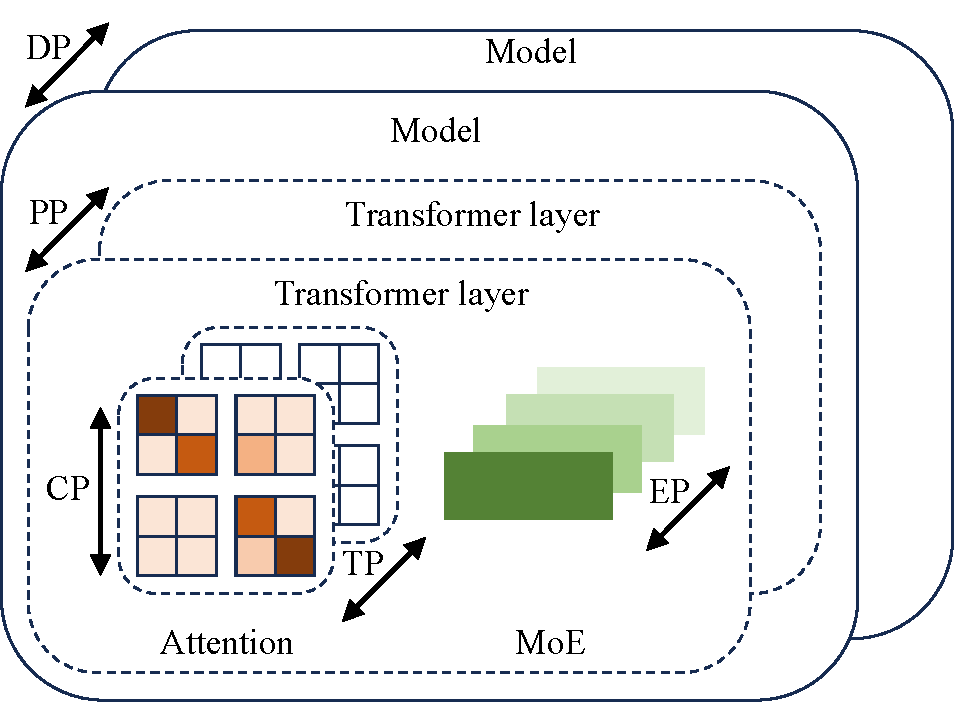
\includegraphics[width=0.49\textwidth]{images/parallelism.pdf}
    \caption{Parallelism overview.}
    \label{fig:megatron_parallelism}
    \vspace{-2ex}  %
\end{wrapfigure}
\paragraph{Efficient Block Diffusion Training} For flexible support of arbitrary block diffusion attention mask, we utilize cuDNN as the backend for the attention mechanism. This approach achieves more than 1.3x end-to-end speedup and over 90\% memory savings in the attention layer compared to the unfused attention implementation in TransformerEngine when training LLaDA2.0-mini. We further apply a zig-zag partitioning strategy to the block diffusion attention mask to achieve effective load balancing across the CP group.

\paragraph{Numerical Stability} During the transition from AR to diffusion models, training can suffer from gradient explosion, especially at high mask ratios within a document. This issue stems from the fact that masked token embeddings are set to zero during AR training, as these tokens are never observed, leading their corresponding weights to gradually decay to zero. A straightforward fix, randomly reinitializing the masked token embeddings upon loading the AR model, may disrupt other well-trained parameters, potentially causing catastrophic forgetting. To mitigate this while preserving pre-trained knowledge, we instead add independent Gaussian noise to the output of the embedding layer for each masked token during the initial iterations of training. This ensures that the L2 norm of the masked token’s embedding remains significant to avoid gradient explosion, thereby stabilizing the training process.

\subsection{Post-Training}
For the post-training phase, we leverage dFactory\footnote{https://github.com/inclusionAI/dFactory}~\citep{dfactory}, a repository providing efficient training recipes for dLLMs. Built upon the VeOmni~\citep{ma2025veomni} distributed training framework, dFactory allows us to effectively implement complex parallelization schemes. Specifically, our setup for fine-tuning LLaDA2.0 combines Data Parallelism (DP) and Expert Parallelism (EP) to ensure scalable and stable training. To further enhance data throughput and hardware utilization, we adopt a data packing strategy analogous to those used in continued pre-training, which concatenates multiple short sequences into a single longer sequence. This integrated approach provides a robust and high-performance infrastructure for the post-training of our model.

\subsection{Inference Engine}
We adapt dInfer\footnote{https://github.com/inclusionAI/dInfer}~\citep{dinfer}--originally built for high-performance diffusion LLM inference--to efficiently support block diffusion inference. This requires the inference engine to leverage optimization techniques traditionally designed for AR models. For instance, the framework can now effectively exploit KV-cache reuse to substantially reduce prefill computation.
As block diffusion inference closely resembles auto-regressive generation in the execution pattern, we also incorporated block diffusion inference support into SGLang\footnote{https://github.com/sgl-project/sglang/issues/12766}~\citep{sglang}, allowing it to benefit from the same class of system-level optimizations designed for AR models. More mature features in dInfer are undergoing to transport to SGLang. 


\paragraph{Inference speed}

\Cref{fig:tps_tparallel} compares the average inference throughput (Tokens Per Second, TPS = \#decoding tokens/\#total-time) of our optimized LLaDA2.0-flash models against state-of-the-art AR models of similar scale on four reasoning and code-generation benchmarks (HumanEval, MBPP, GSM8K, and CRUXEval). All models are evaluated under a consistent generation setup. For diffusion-based models (LLaDA2.0-flash and LLaDA2.0-flash-CAP), we adopt a threshold decoder with a threshold of 0.95. The AR baselines (Ling-flash-2.0 and Qwen3-30B-A3B-Instruct-2507) are deployed using SGLang, while the diffusion models are served with dInfer, ensuring fair performance comparison in real inference environments.
As shown, LLaDA2.0-flash-CAP reaches 535 TPS, outperforming the standard LLaDA2.0-flash (383 TPS) and providing up to 2.1× speed-up over the AR baselines (256 TPS and 237 TPS).
